\chapter{Q02}
\emph{Q2: Describe the possible energy sources for WSN nodes? What are the pro
and cons of the different sources? Explain how the energy drawn from the energy
source(s) can be measured and calculated?}

\section{Energy}

\subsection{Goal}
\begin{description}
\item provide as much energy as possible at smallest cost$\slash$volume$\slash$weight$\slash$recharge time$\slash$longevity.
\end{description}

\subsection{Storage}
\begin{description}
\item Primary batteries. Not rechargeable.
\item Secondary batteries. Rechargeable $\Rightarrow$ energy harvesting.
\end{description}

\subsection{Requirements}
\begin{description}
\item Low self-discharge.
\item Long shelf-life.
\item Capacity under load.
\item Voltage stability (Avoid DC-DC conversion.)
\end{description}

\begin{figure}[h]
  \centering
    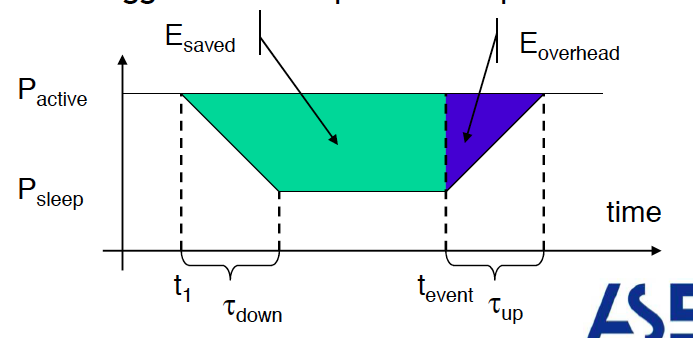
\includegraphics[scale=0.5]{img/EnergySources-DutyCycling.png}
    \caption{Duty cycling.}
\end{figure}

\subsection{Shunt resistor}

\begin{align*}
  U_{shunt}(t) &= R \times I(t) \\
  U_{mote}(t) &= U_{battery}(t) \times U_{shunt}(t) \\
  P_{mote} (t) &= U_{mote}(t) \times I(t) \\
  E_{mote} &= \int_{t_o}^{t_1} U_{mote}(t) \times I(t) dt
\end{align*}

%%% Local Variables: 
%%% mode: latex
%%% TeX-master: "../master"
%%% End: 
